% Copyright (c) 2014,2016 Casper Ti. Vector
% Public domain.

\chapter{研究動機}
%\pkuthssffaq % 中文测试文字。
	\section{密碼貨幣的發展}
	追溯著加密貨幣市場的演進,於2009年時,比特幣並非第一個密碼貨幣,在比特幣之前已經有著很多的類似的密碼貨幣開發實驗,但是一直無法做出一個穩定點對點式的電子現金系統,至於製作貧頸會在後段章節中闡述。在比特幣穩定發展之後,有著許多對比特幣有興趣的研究者,以穩定的比特幣系統為基礎修改了許多基本的協議。於2011年相繼創造出了貨幣就稱之為山寨幣,山寨幣早期較為著名的有萊特幣(LiteCoin,LTC)\parencite{litecoin}、狗幣(DogeCoin,DOGE)\parencite{dogecoin}、域名幣(NameCoin,NMC)\parencite{namecoin},於2014年也有人認為比特幣挖礦使用到了大量的哈希運算,這樣的大量運算也浪費了許多的社費資源,努力的開發具有意義的工作量證明挖礦算法較為著名的有素數幣(Primecoin,XPM)\parencite{primecoin}。 於2015年底也誕生了現在最為著名的以太坊經典(Ethereum Classic,ETC)\parencite{ethereumclassic}、以太坊(Ethereum,ETH)\parencite{ethereum},使得區塊鏈技術不再僅僅只是一個點對點的電子現金系統,以太坊最重大突破設計在於將編程語言虛擬機,移植到了區塊鏈架構上,也創造出了屬於乙太坊的編程語言Solidity,使得再以太坊的虛擬機當中,可以用Solidity創建智能合約,合約可以建構去中心化的應用程序,如去中心化的交易所。

	\section{密碼貨幣市場(Cryptocurrency Market)}
	密碼貨幣最具代表性的是比特幣,但除了比特幣之外也有著許多模仿比特幣的密碼貨幣,有的是為了利益,有的是鑒於比特幣的各種不完美,希望可以解決比特幣不足之處。密碼貨幣市場中有成千上萬種的密碼貨幣,較為著名的密碼貨幣會在Cryptocurrency Market Capitalizations\parencite{CryptocurrencyMarketCapitalizations}的排行榜中出現,截至2018年2月8日該排行榜已經收入了1510種密碼貨幣。在Cryptocurrency Market Capitalizations統計的數據當中,可知整體的密碼貨幣市場,如下圖\ref{TotalMarketCapitalization}所示,於2018年1月7日創下了歷史新高,密碼貨幣市場的總市值也高達了829,579,000,000美金,相當於五兆人民幣的總市值。

		\begin{figure}[htbp]
			\centering
			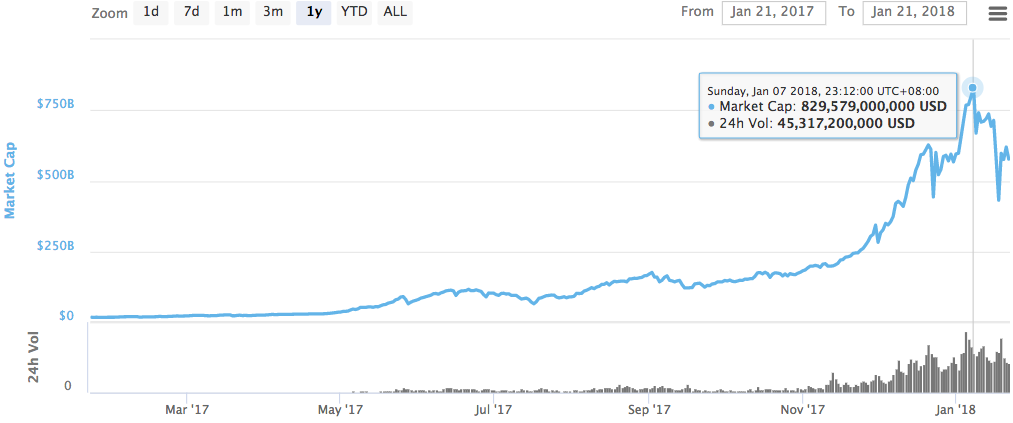
\includegraphics[width = .9\textwidth]{TotalMarketCapitalization.png}
			\caption{Total Market Capitalization\parencite{TotalMarketCapitalization}}\label{TotalMarketCapitalization}
		\end{figure}

	\section{密碼貨幣的優勢}

	\section{密碼貨幣的劣勢}
% vim:ts=4:sw=4
